%\section{Preliminaries}
%This section presents the process of CDA-AL, as well as representative data poisoning attacks developed for static (non-drift) learning environments.

\section{Background: Concept Drift Adaptation with Active Learning}
\label{Sec: Concept Drift Adaptation}

CDA-AL is a paradigm that enhances model performance by identifying high-uncertainty samples from the testing data~\cite{2023-Usenix-chenyizhen,park2016active,vzliobaite2013active}.
%\begin{figure}[t]
%	\centering
%	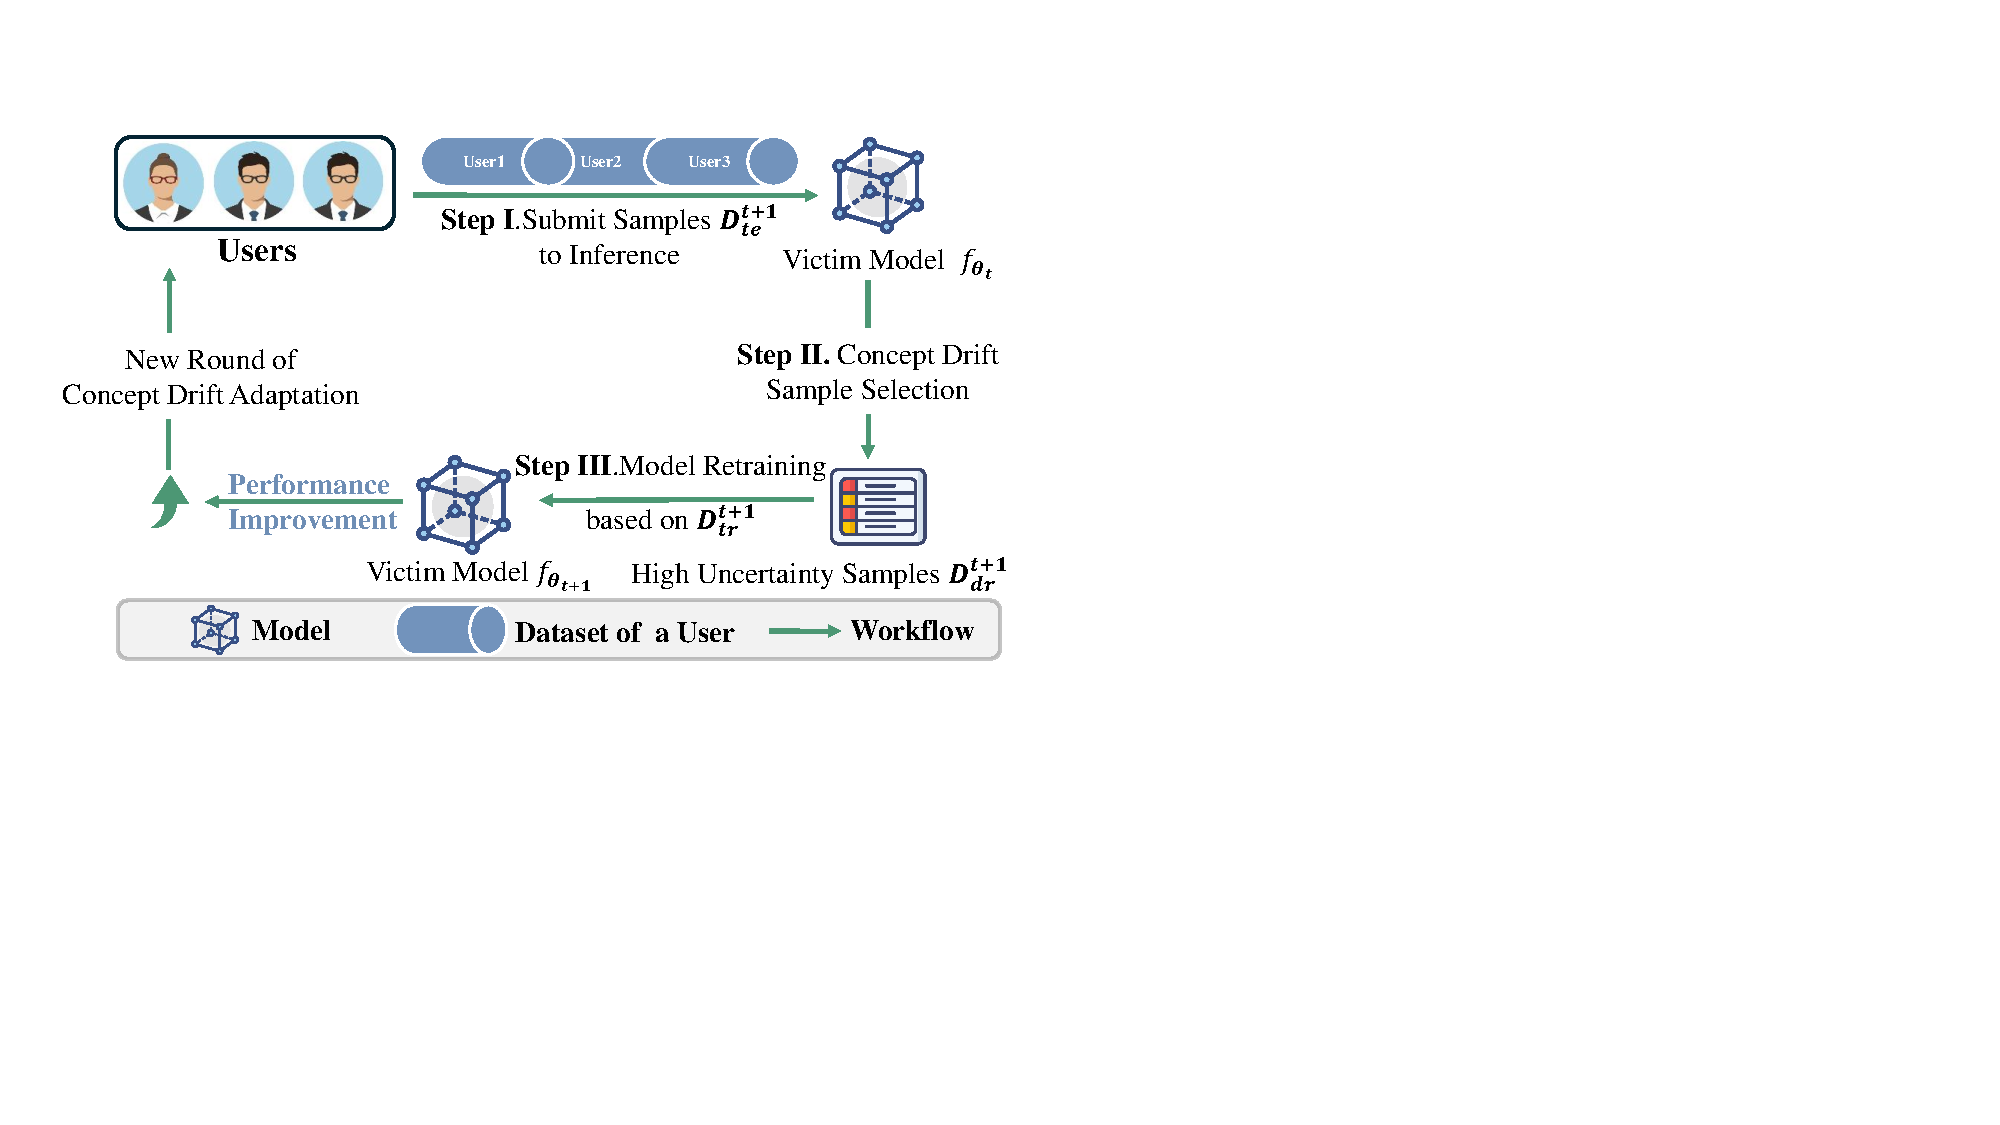
\includegraphics[width=\linewidth,keepaspectratio]{Graph/Intro_graph/Background/Concept_Drift_Adaptation_Based_Active_Learning_2025_3_27_15_23.pdf}
%	\caption{Concept drift adaptation based active learning}
%	\label{fig: CDA-AL-1}
%\end{figure}
%The overall process is illustrated in Figure~\ref{fig: CDA-AL-1}.
For consistency, we refer to the concept drift adaptation model as the victim model throughout this paper.
The entire concept drift process is composed of multiple concept drift cycles.
%The number of concept drift cycles is set to $n$ in our subsequent discussions.
Let $f_{\bm{\theta}_{n}}$ denote the victim model trained on the training data $\bm{D}^{n}_{tr}$ in concept drift cycle $n$.
$\bm{\theta}_{n}$ denotes the retrained model parameters at the end of concept drift cycle $n$, while $\bm{D}^{n}_{tr}$ refers to the updated training dataset used by the victim model during that cycle.
The unlabeled testing dataset $\bm{D}_{te}^{n}$ comprises all samples collected by the victim model throughout concept drift cycle $n$.
For concept drift cycle $n$, the concept drift adaptation process generally consists of three steps:

\emph{Step I}: Victim Model $f_{\bm{\theta}_{n-1}}$ performs inference on the input $\bm{\mathrm{x}}_{i} \in \bm{D}_{te}^{n}$ and obtain the classification confidence vector $\bm{\mathrm{c}}_{i} = f_{\bm{\theta}_{n-1}} \left( \bm{\mathrm{x}}_{i} \right)$.
	The different dimensions of $\bm{\mathrm{c}}_{i}$ indicate the model's confidence that the input $\bm{\mathrm{x}}_{i}$ belongs to a specific sample label. 
	The label with the highest confidence is selected as the predicted label $\overline{y}_{i}$ on the input $\bm{\mathrm{x}}_{i}$.

\emph{Step II}: %Based on the confidence vector $\bm{\mathrm{c}}_{i}$ obtained in the previous step, 
	The uncertainty score $\bm{\mathrm{u}}_{i}$ of $\bm{\mathrm{x}}_{i}$ is measured.
	For example, uncertainty can be measured as one minus the maximum softmax output of the network~\cite{2023-Usenix-chenyizhen}:
$\bm{\mathrm{u}}_{i} = 1-\max(\bm{\mathrm{c}}_{i},1-\bm{\mathrm{c}}_{i})$.
	We use $uncer()$ to denote uncertainty measures in the following discussion.
	
\emph{Step III}: High-uncertainty samples are selected from the testing data $\bm{D}_{te}^{n}$ as concept drift samples $\bm{D}_{dr}^{n}$.
	The size of $\bm{D}_{dr}^{n}$ is determined by the manual labeling capacity, referred to as the labeling budget $\beta$.
	Then, the concept drift data $\bm{D}_{dr}^{n}$ is manually labeled to get the ground truth label and added to the existing training data $\bm{D}^{n-1}_{tr}$ to form an updated training data $\bm{D}^{n}_{tr} = \bm{D}_{tr}^{n-1} \cup \bm{D}_{dr}^{n}$.
	The victim model $f_{\bm{\theta}_{n-1}}$ is then retrained on the updated training data $\bm{D}^{n}_{tr}$ to yield an updated model $f_{\bm{\theta}_{n}}$, as described in Equation~\ref{active learning loss}.
	\begin{equation}
		\begin{aligned}
			\bm{\theta}_{n} = \arg\min_{\bm{\theta}_{n-1}} \sum_{\bm{\mathrm{x}}_{i} \in \bm{D}^{n}_{tr}} \mathcal{L} \left( f_{\bm{\theta}_{n-1}}\left( \bm{\mathrm{x}}_{i}\right) , y_{i}  \right) \\
		\end{aligned}
		\label{active learning loss}
	\end{equation}


%\textbf{didn't you already mention this??? what is the point of this paragraph??}
%In this paper, we refer to the samples selected by the uncertainty-based selection strategy as concept drift samples, although they may not be directly affected by drift.
%Uncertainty can also result from other factors, such as when samples lie near the decision boundary in a stable distribution.
%Following prior work~\cite{2023-Usenix-chenyizhen}, we do not explicitly distinguish these samples in the following discussion since such differentiation pertains to concept drift detection rather than adaptation.

\begin{comment}
\subsection{Data Poisoning Attacks}
\label{Sec: Data Poisoning Attacks}

In data poisoning attacks, the attacker constructs poisoned data to degrade the performance of the victim model.
The most common strategy is to inject poisoned samples into the victim model’s training dataset.
As noted by Tian et al.~\cite{2022-ACM-Computing-Survey-Poisoning-attacks-and-countermeasures-in-ML} and Wang et al.~\cite{2022-ACM-Computing-Survey-Threats-to-training}, such attacks are generally categorized as targeted or untargeted.
Untargeted poisoning attacks aim to hinder the convergence of the victim model and eventually lead to denial-of-service~\cite{pmlr-v20-biggio11,2023-AAAI-yuuntargeted,wang2023analysis}.
The challenge with untargeted attacks is that they aim to degrade the performance across all data~\cite{2024-CCS-Phantom}.
Therefore, the effect of poisoned samples must outweigh that of the clean training data.
In contrast, targeted poisoning attacks aim to manipulate the victim model into making incorrect predictions on specific inputs~\cite{2024-TIFS-Backdoor-Contrastive-Learning,2021-Usenix-Poisoning-Attack-Explanation-guided-Backdoor,2023-SP-backdoor-attack}.
The inputs for which the model’s predictions are compromised are called attack targets. 
To launch a targeted poisoning attack, an adversary needs to
inject malicious knowledge into the training data while keeping other knowledge unaffected~\cite{2022-ACM-Computing-Survey-Poisoning-attacks-and-countermeasures-in-ML}.
\end{comment}
